\documentclass{article}
%\usepackage{geometry}
% \geometry{top = 1in, bottom = 1in, left = 1in, right = 1in}
\usepackage[top = 0.7in, bottom = 0.7in, left = 0.7in, right = 0.7in]{geometry}
\usepackage{amsmath,amssymb,amsthm,mathrsfs}
\usepackage{graphicx}
\usepackage{bm}
\usepackage{float}
\usepackage[font=footnotesize,labelfont=bf]{caption}

\usepackage{fancyhdr}
\pagestyle{fancy}
\rhead{\footnotesize {07/28/2012 ; MESA version 4028} }
\chead{\footnotesize {Authors: Jared Brooks, Lars Bildsten, Bill Paxton} }
\lhead{\footnotesize {mesa/star/test\_suite/wd2} }

\begin{document}
	
	\begin{center}
		\begin{Large}
			\textbf{WD2}\\
		\end{Large}
	\end{center}
	

        This test is to show a 1 $M_\odot$ white dwarf undergoing two nova bursts and maintaining steady hydrogen burning thereafter.  The test should be cut off when the mass reaches $1.00005$ $M_\odot$ (\texttt{star\_mass\_max\_limit = 1.00005d0}).\\

        The inlist for this test loads a pre-saved white dwarf and begins accreting material at a rate of $2\times10^{-7}$ $M_\odot$/yr (\texttt{mass\_change = 2d-7}), composition of the accreted material listed below.\\

	\noindent Accreted Material composition (mass fractions):
        \begin{itemize}
        \item $^1$H: 0.749
        \item $^3$He: 2.9291e-5
        \item $^4$He: 0.237
        \end{itemize}

        The following few plots show the activity of the white dwarf right before, during, and after the nova events.  Here is a plot (figure \ref{fig:1}) of the mass of the white dwarf against the age of the model showing the first nova at about 64 years and the second at about 116 years, indicated by the sudden mass loss.  The figure to the right (figure \ref{fig:4}), which plots the total hydrogen mass against the age of the model, showing that all the hydrogen accreted after the novae is being consumed by steady hydrogen burning.

	\begin{figure}[H]
          \begin{minipage}[b]{0.5\linewidth}
	    \centering
	    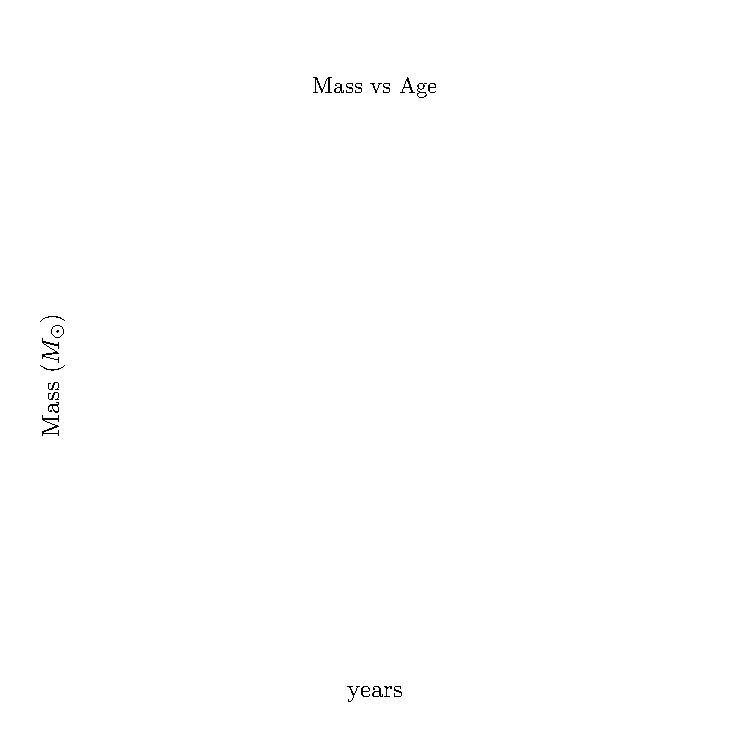
\includegraphics[width = 3.8in]{/Users/jaredbrooks/wd2/plots_out/Mass_vs_Age.pdf}
	    \caption{Constant mass accretion rate with two novae that cause mass loss}
	    \label{fig:1}
          \end{minipage}
          \hspace{0cm}
          \begin{minipage}[b]{0.5\linewidth}
            \centering
            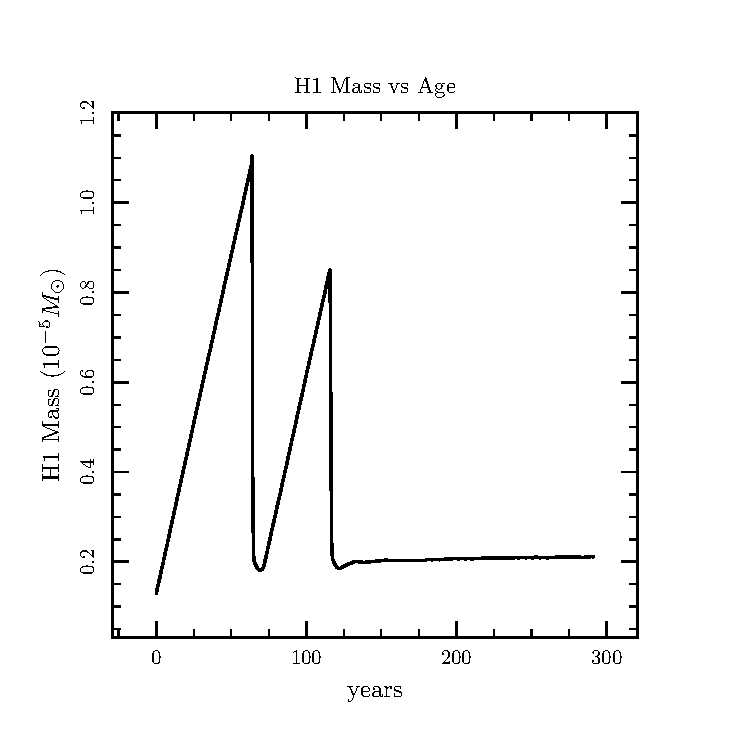
\includegraphics[width = 3.8in]{/Users/jaredbrooks/wd2/plots_out/H1_Mass_vs_Age.pdf}
            \caption{Hydrogen mass consumed in two novae, followed by steady burning}
            \label{fig:4}
          \end{minipage}
	\end{figure}
        
        \pagebreak

        These novae events take place on the surface of the white dwarf, indicated by this burning rate profile given during the first nova at 64 years (figure \ref{fig:5}) shown to the left.  To the right is an abundance profile from the end of the run (figure \ref{fig:7}).  Both profiles are plotted against logxq, where logxq = log(1-q) and q is the fraction of star mass interior to outer boundary of each zone, moving outwards from the core.

        \begin{figure}[H]
          \begin{minipage}[b]{0.5\linewidth}
            \centering
            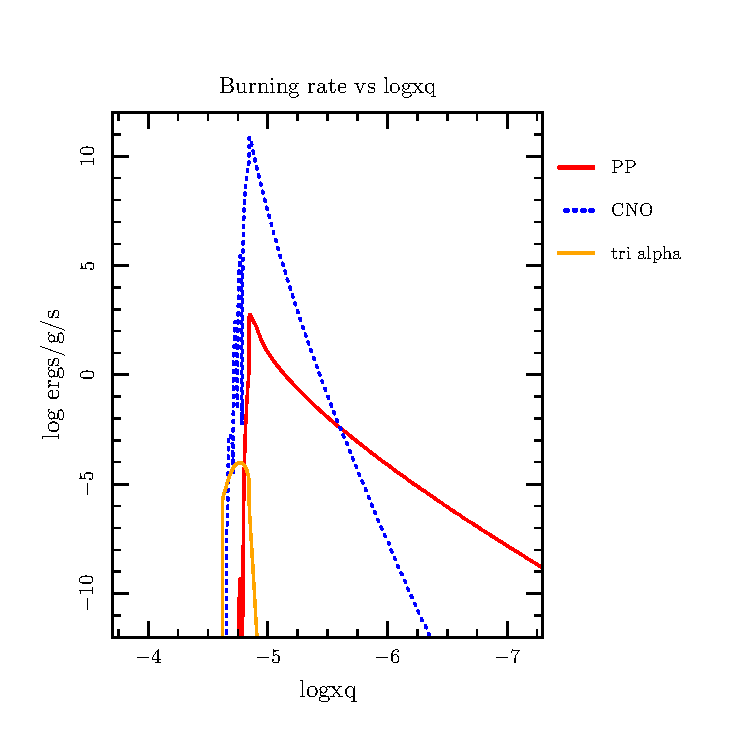
\includegraphics[width = 3.7in]{/Users/jaredbrooks/wd2/plots_out/Burning_rate_vs_logxq_5.pdf}
            \caption{Burning rate profile during first nova}
            \label{fig:5}
          \end{minipage}
          \hspace{0cm}
          \begin{minipage}[b]{0.5\linewidth}
            \centering
            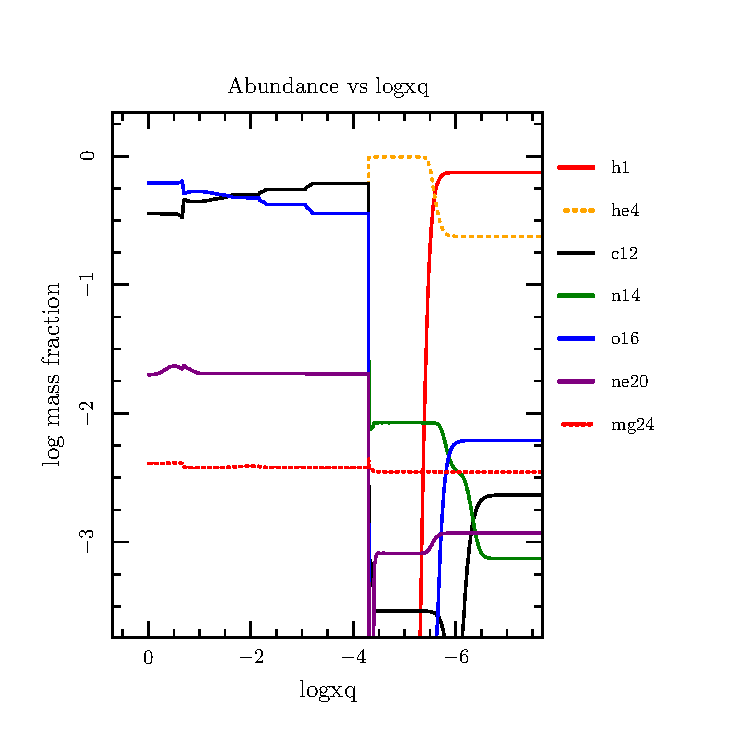
\includegraphics[width = 3.7in]{/Users/jaredbrooks/wd2/plots_out/Abundance_vs_logxq_12.pdf}
            \caption{Abundance profile from end of run}
            \label{fig:7}
          \end{minipage}
          \end{figure}

        This rapid burning during the novae give sharp peaks in hydrogen luminosity (figure \ref{fig:2}) and the released heat causes jumps in the radius (figure \ref{fig:3}).
        
        \begin{figure}[H]
          \begin{minipage}[b]{0.5\linewidth}
            \centering
            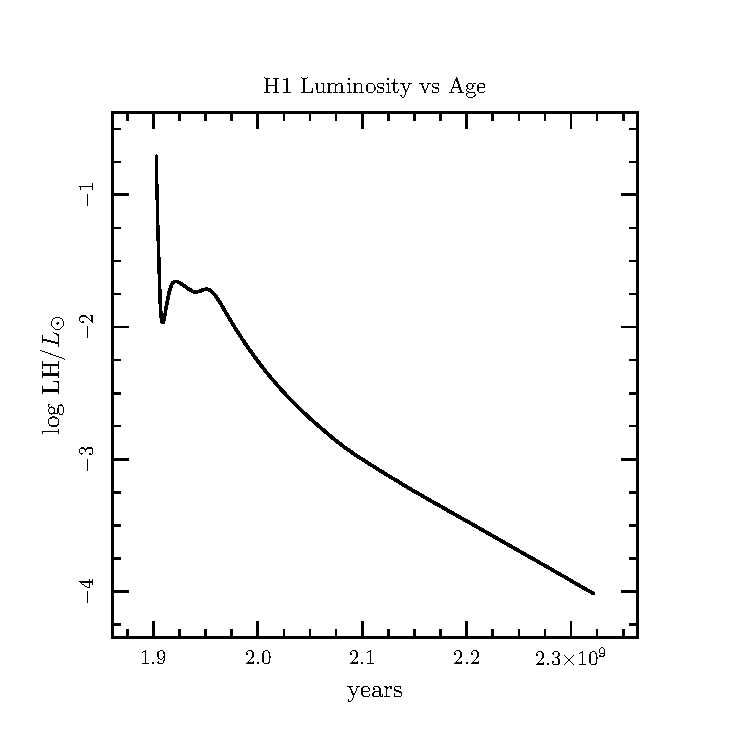
\includegraphics[width = 3.7in]{/Users/jaredbrooks/wd2/plots_out/H1_Luminosity_vs_Age.pdf}
            \caption{\footnotesize Hydrogen luminosity peaks caused by novae}
            \label{fig:2}
          \end{minipage}
          \hspace{0cm}
          \begin{minipage}[b]{0.5\linewidth}
            \centering
            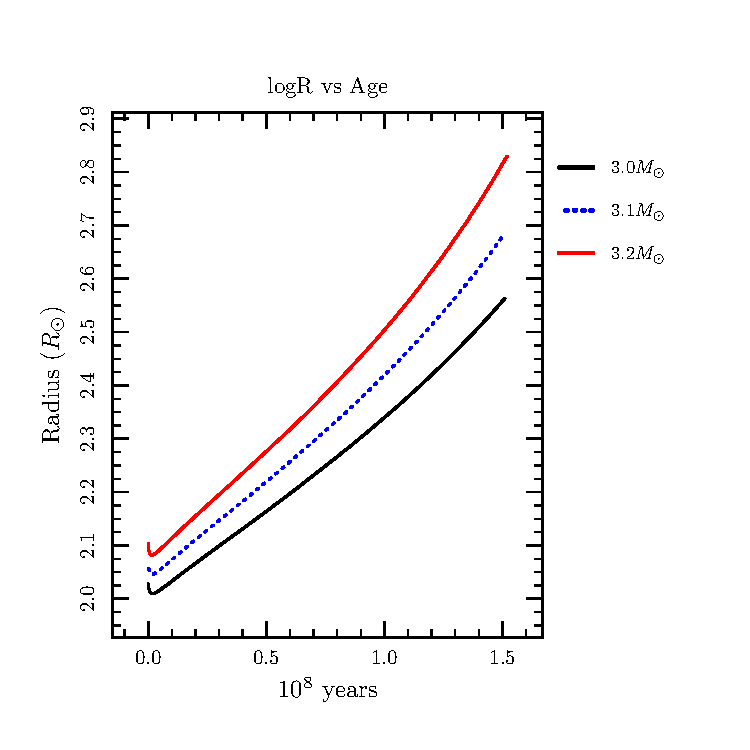
\includegraphics[width = 3.7in]{/Users/jaredbrooks/wd2/plots_out/logR_vs_Age.pdf}
            \caption{\footnotesize Radius peaks caused by heat release from novae}
            \label{fig:3}
          \end{minipage}
        \end{figure}

        \pagebreak

        This final plot (figure \ref{fig:6}) shows a few internal \texttt{MESA} variables, such as the size of the time-step, the number of zones, and the number of retries against the model number in order to give some understanding of how hard \texttt{MESA} is working throughout the run and where some areas of problems/interest might be.

        \begin{figure}[H]
          \centering
          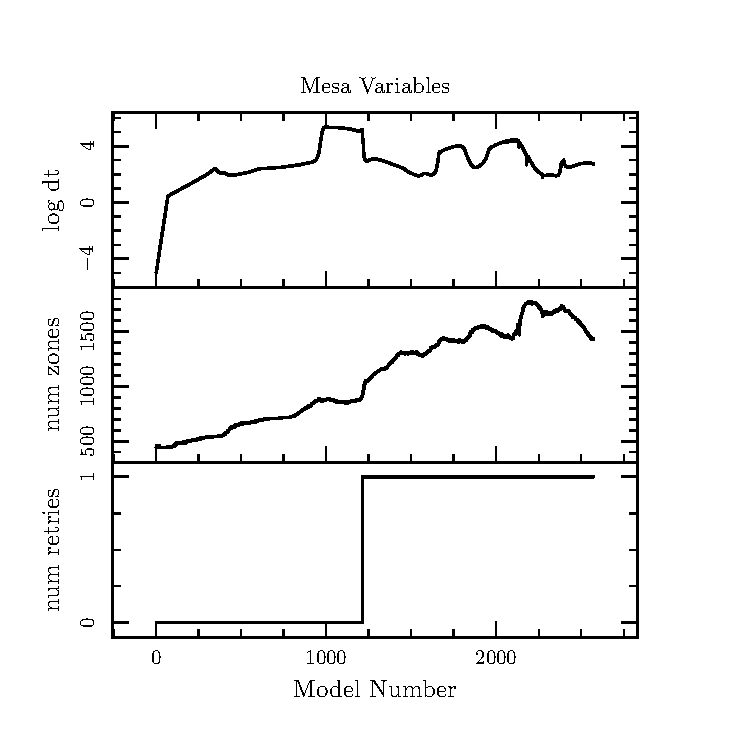
\includegraphics[width = 5in]{/Users/jaredbrooks/wd2/plots_out/Mesa_Variables.pdf}
          \caption{\texttt{MESA} variables plotted against model number show how hard \texttt{MESA} is working}
          \label{fig:6}
        \end{figure}

\end{document}


